\documentclass[12pt]{article}

\usepackage[pdftex]{graphicx}
\usepackage{cancel}
\usepackage[margin=4cm]{geometry}
\usepackage[hidelinks]{hyperref}
\usepackage{fancyhdr}
\usepackage{amsmath}
\usepackage{amsfonts}
\usepackage{dirtytalk}
\usepackage{parskip}

\newcommand\tab[1][1cm]{\hspace*{#1}}
\newcommand{\HRule}{\rule{\linewidth}{0.5mm}}
\newcommand{\course}{COMS 474}

\setcounter{secnumdepth}{0} % Disable section/subsection numbering
\hyphenpenalty 10000 % Prevent words from being broken over multiple lines
\exhyphenpenalty 10000 % Prevent words from being broken over multiple lines

% Margins
\topmargin=-0.45in
\evensidemargin=0in
\oddsidemargin=0in
\textwidth=6.5in
\textheight=9.0in
\headsep=0.25in
\title{ \course \\\large Homework 8 }
\author{ Haadi Majeed }
\date{Spring 2022}


\pagestyle{fancy}
\fancyhead{}
\fancyfoot{}
\lhead{\course}
\chead{Haadi Majeed}
\rhead{Page \thepage}

\begin{document}
\maketitle
\pagebreak

% Optional TOC
%\tableofcontents
\pagebreak
\section{Problem 1}
 [15 points; 3 each]\\
Consider the following data set. There are two classes for
Y (mapped to \{-1, +1\}). There is one feature X that can be used for prediction.
\begin{center}
    \begin{tabular}{ |c|c| }
        \hline
        Y  & X  \\
        \hline
        -1 & 6  \\
        \hline
        -1 & 7  \\
        \hline
        -1 & 11 \\
        \hline
        +1 & 9  \\
        \hline
        +1 & 13 \\
        \hline
        +1 & 14 \\
        \hline
    \end{tabular}
\end{center}
\subsection{A}
Draw the scatter plot of the data by hand.\\
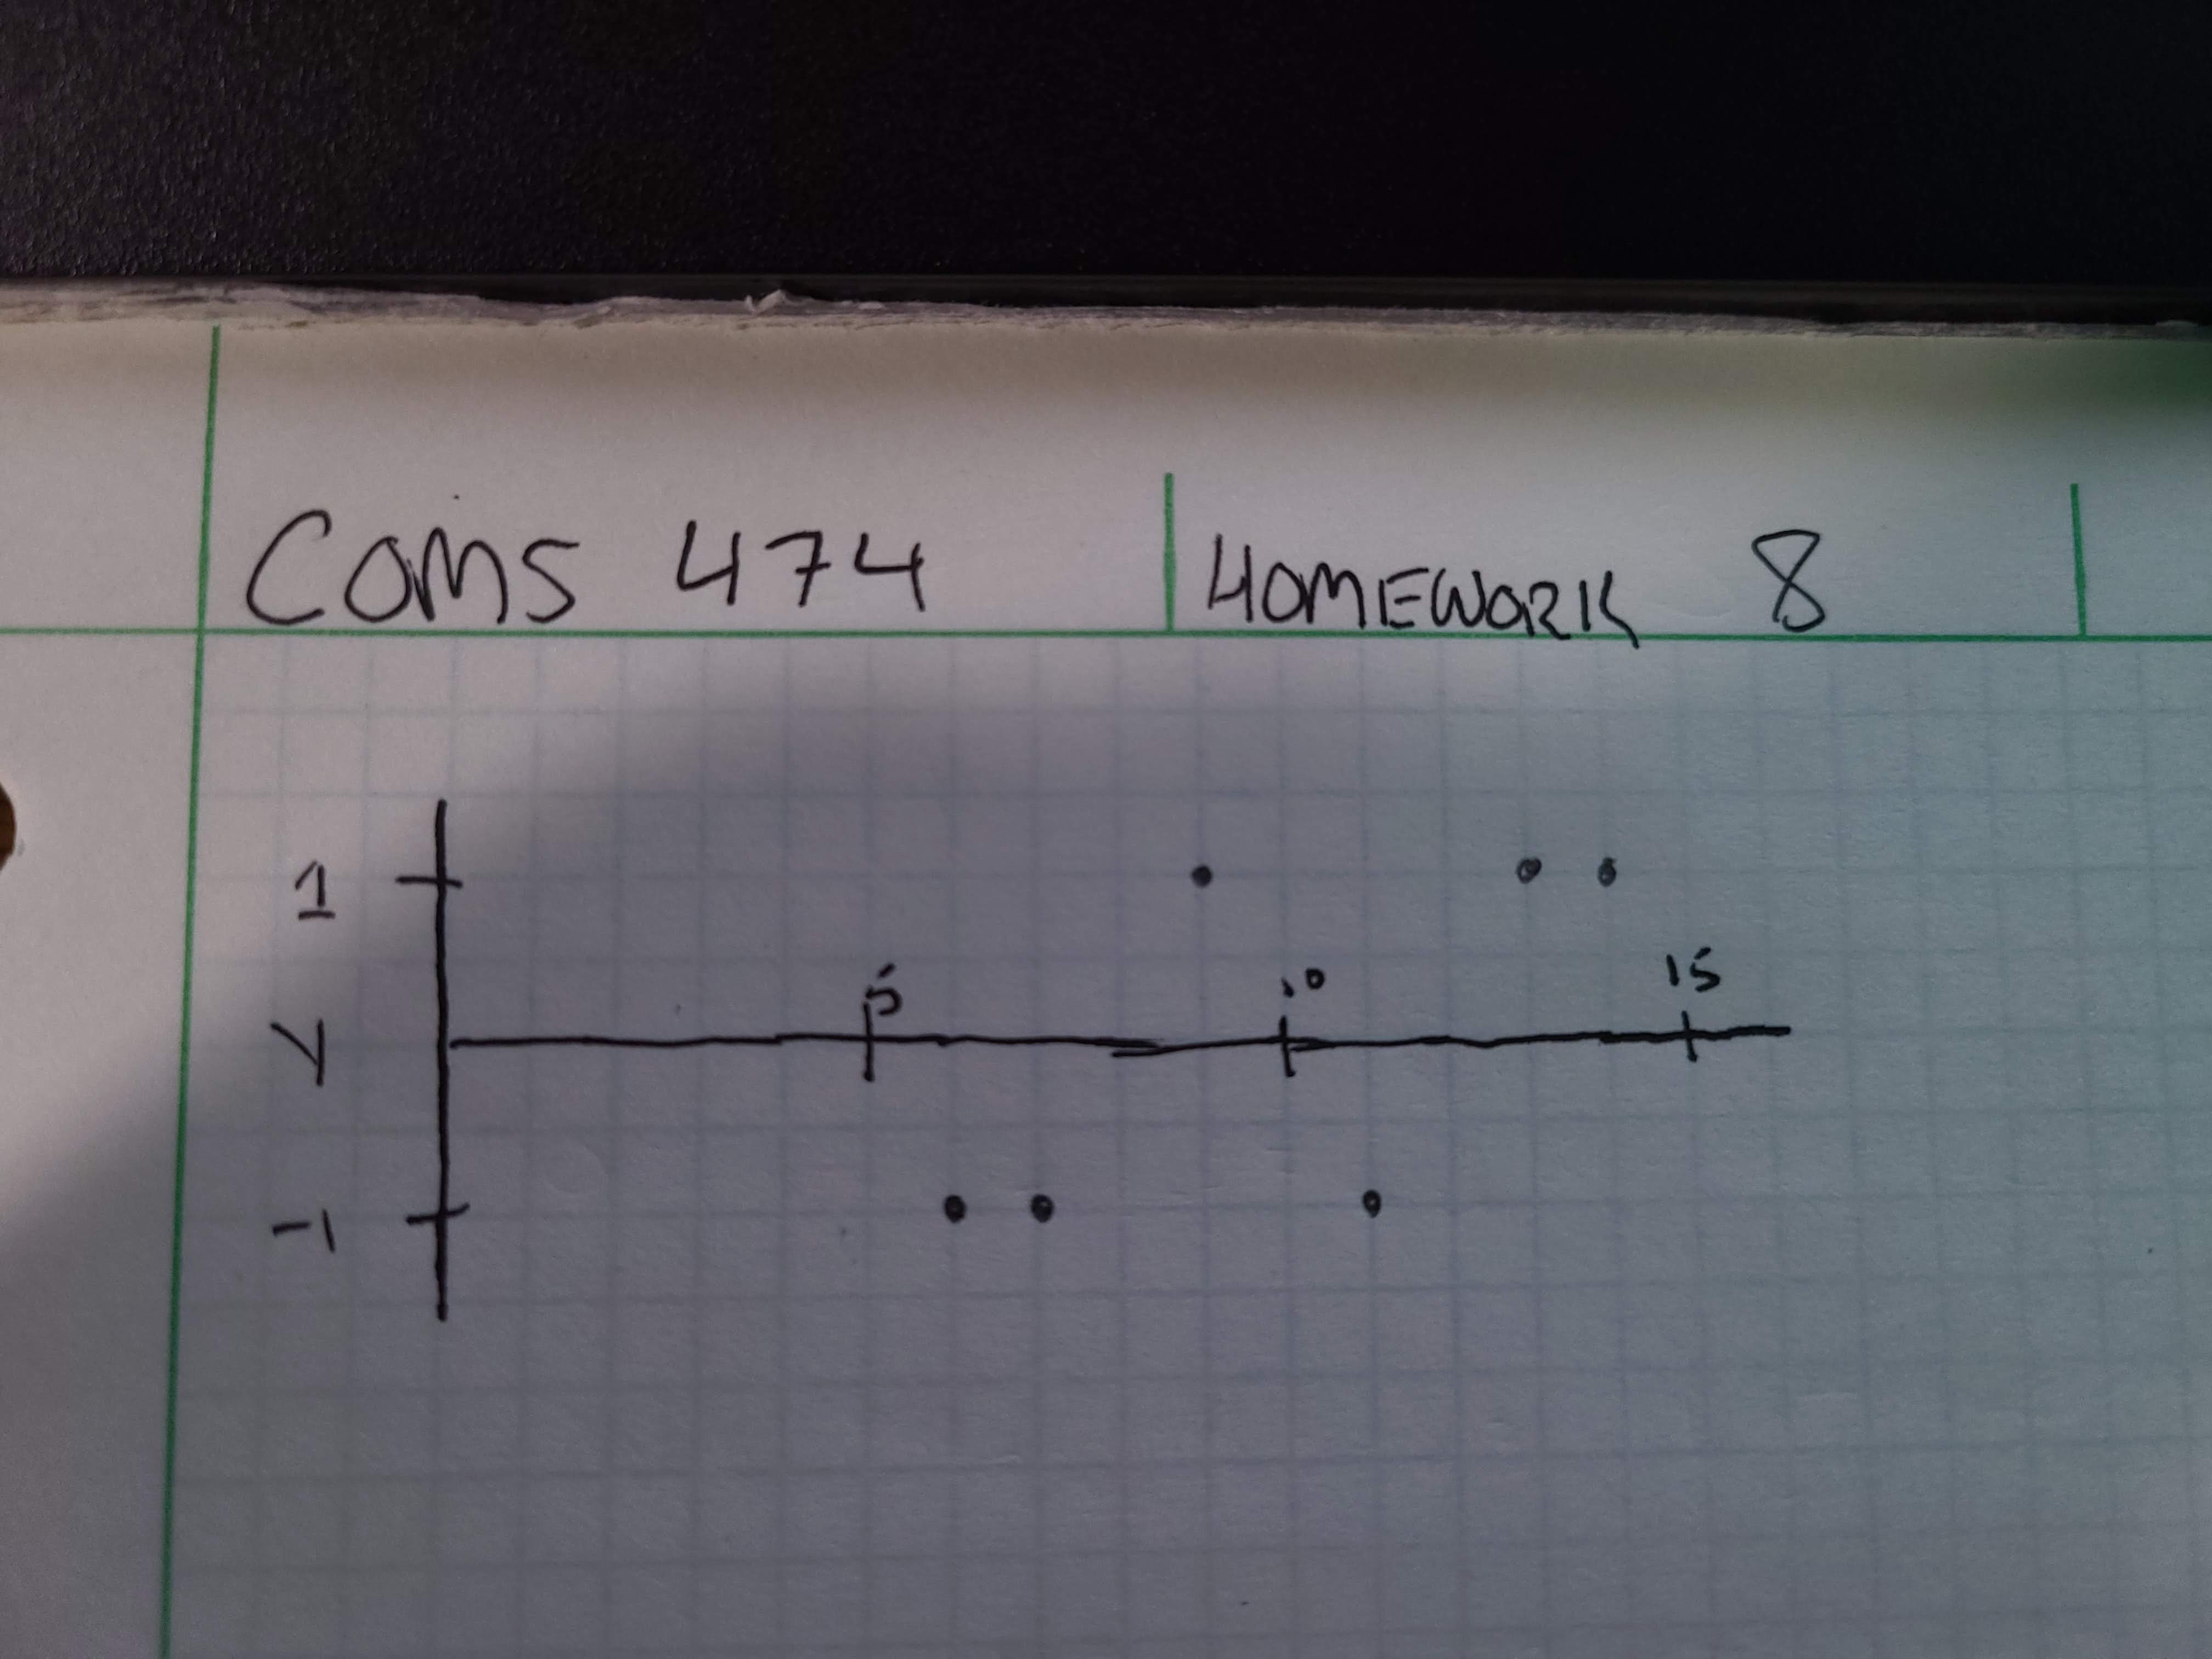
\includegraphics[width=1\textwidth]{p1.a.jpg}
\subsection{B}
Sketch the prediction function $\hat{Y}(x)$ for the $k = 1$ nearest neighbour classifier on the scatter plot. Briefly explain your process.\\
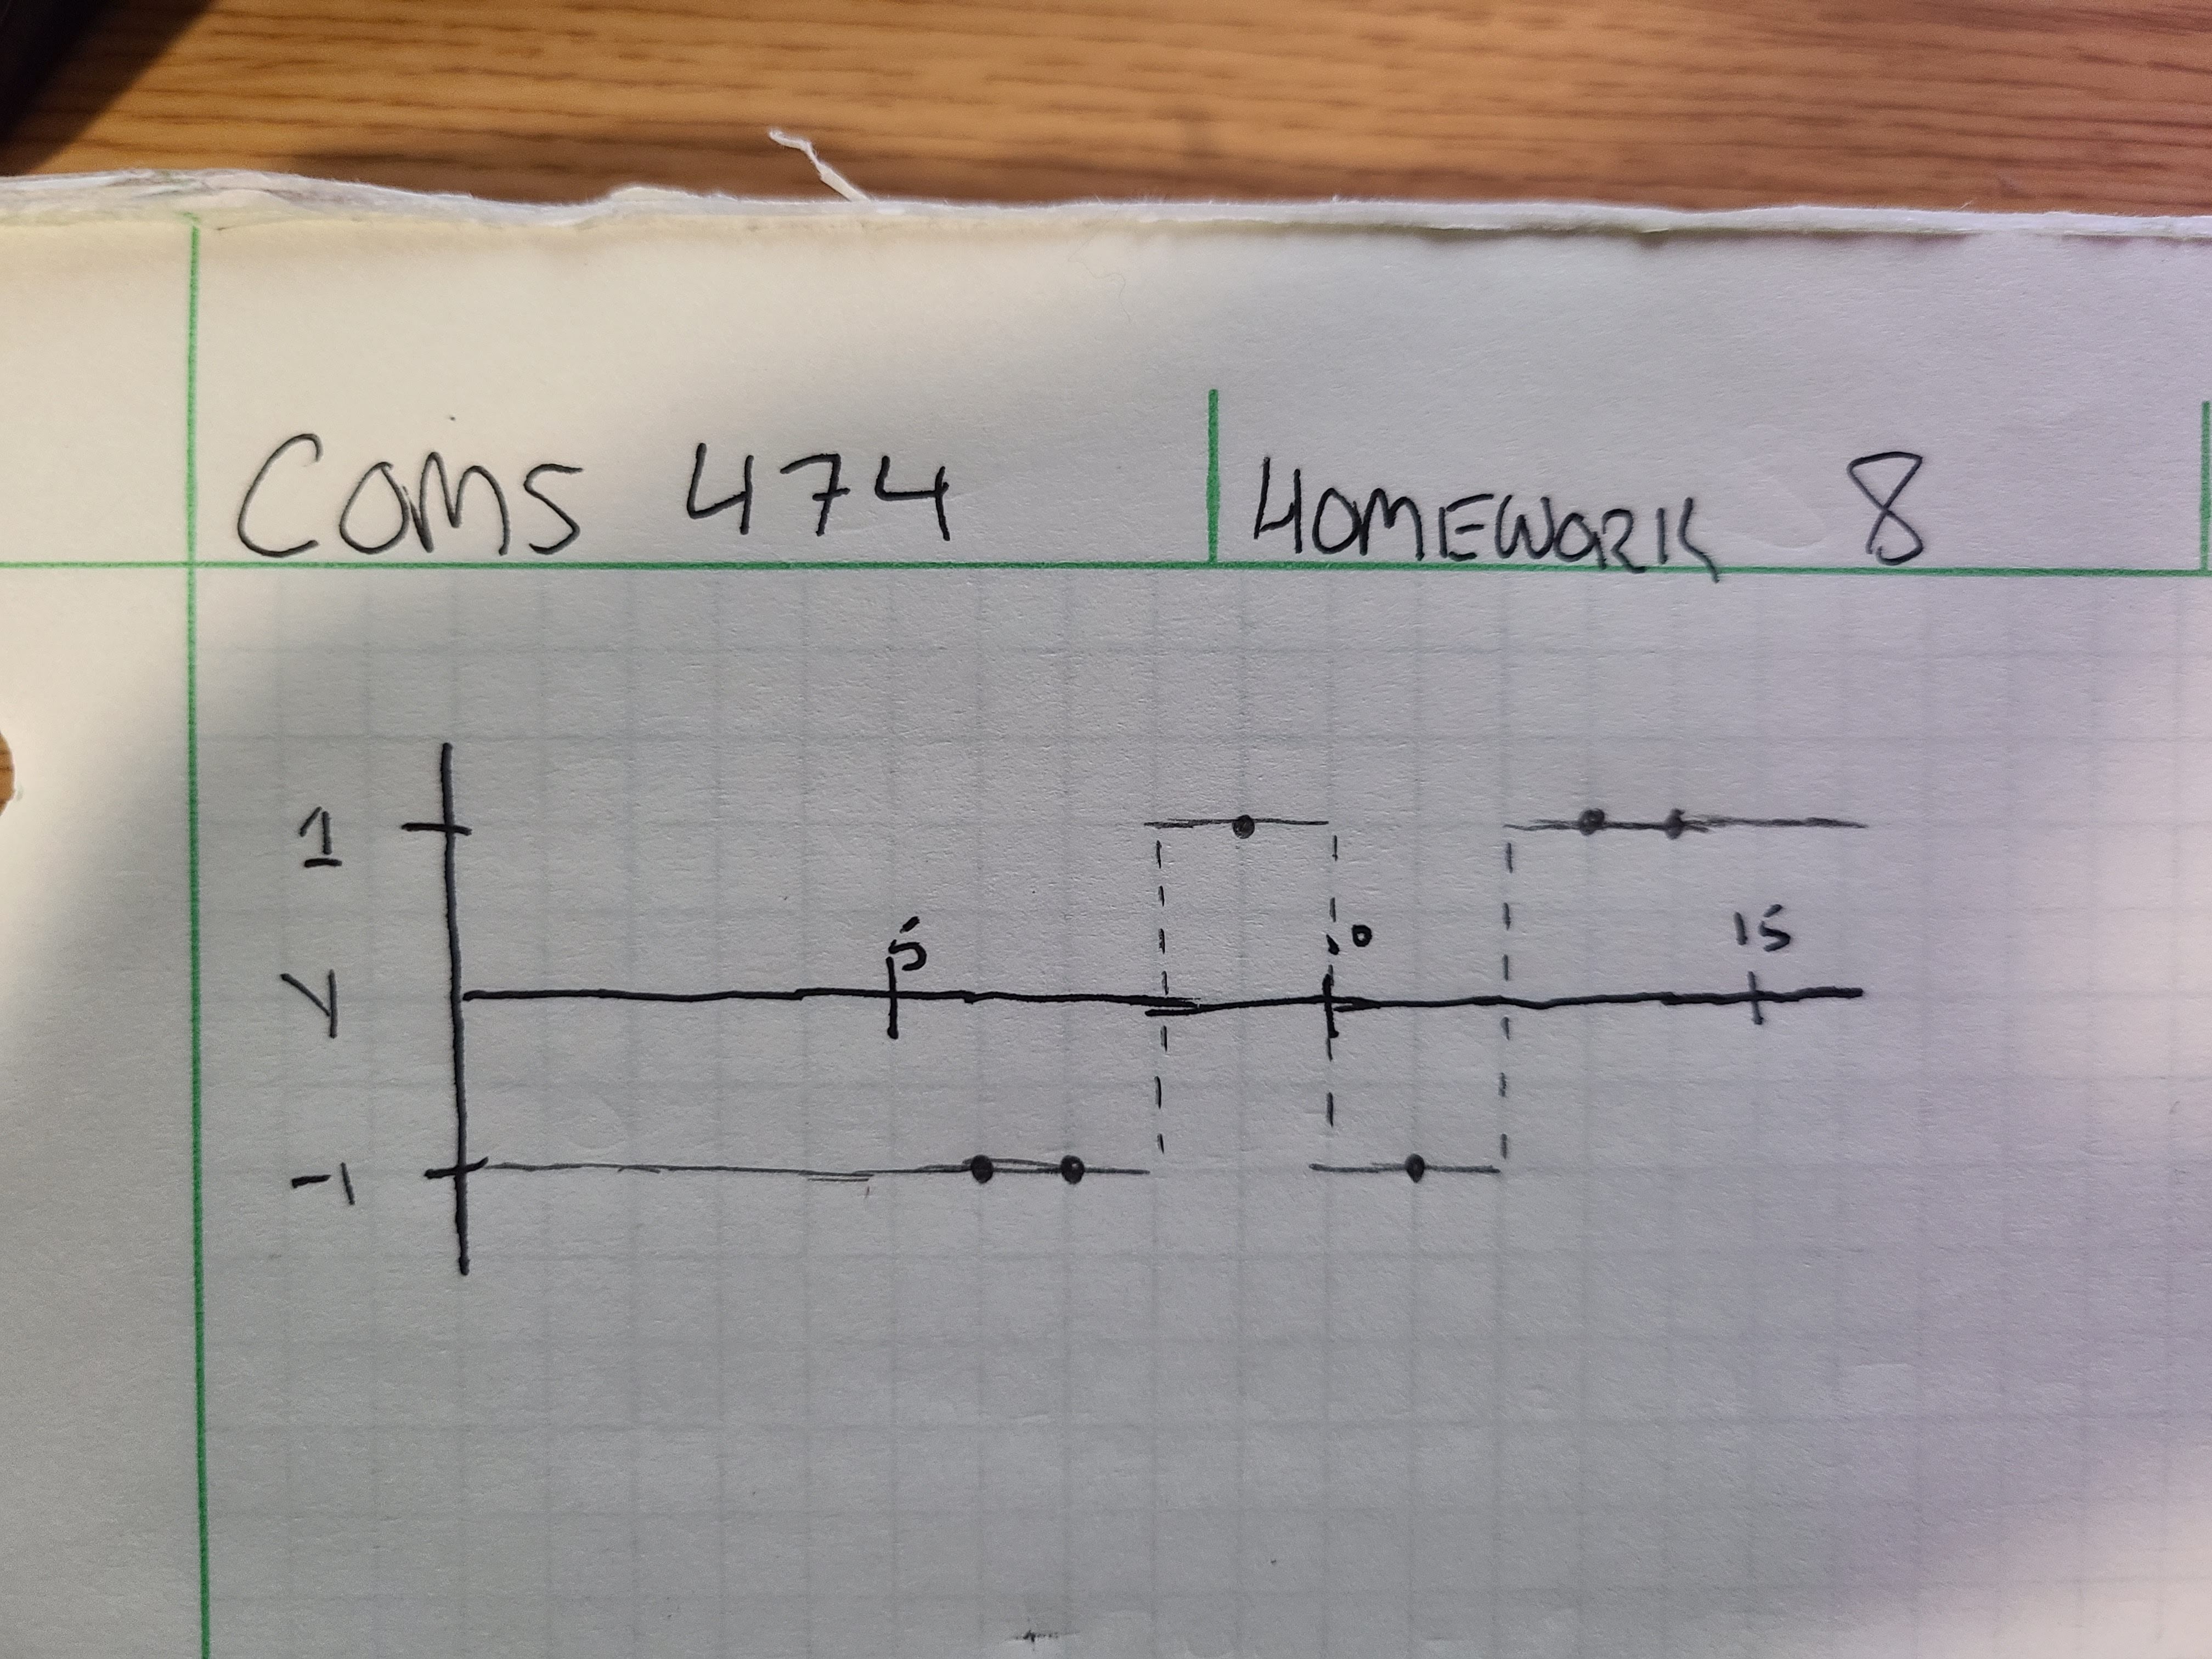
\includegraphics[width=1\textwidth]{p1.b.jpg}
\subsection{C}
Sketch the prediction function $\hat{Y}(x)$ for the $k = 3$ nearest neighbour classifier on the scatter plot. Briefly explain your process.\\
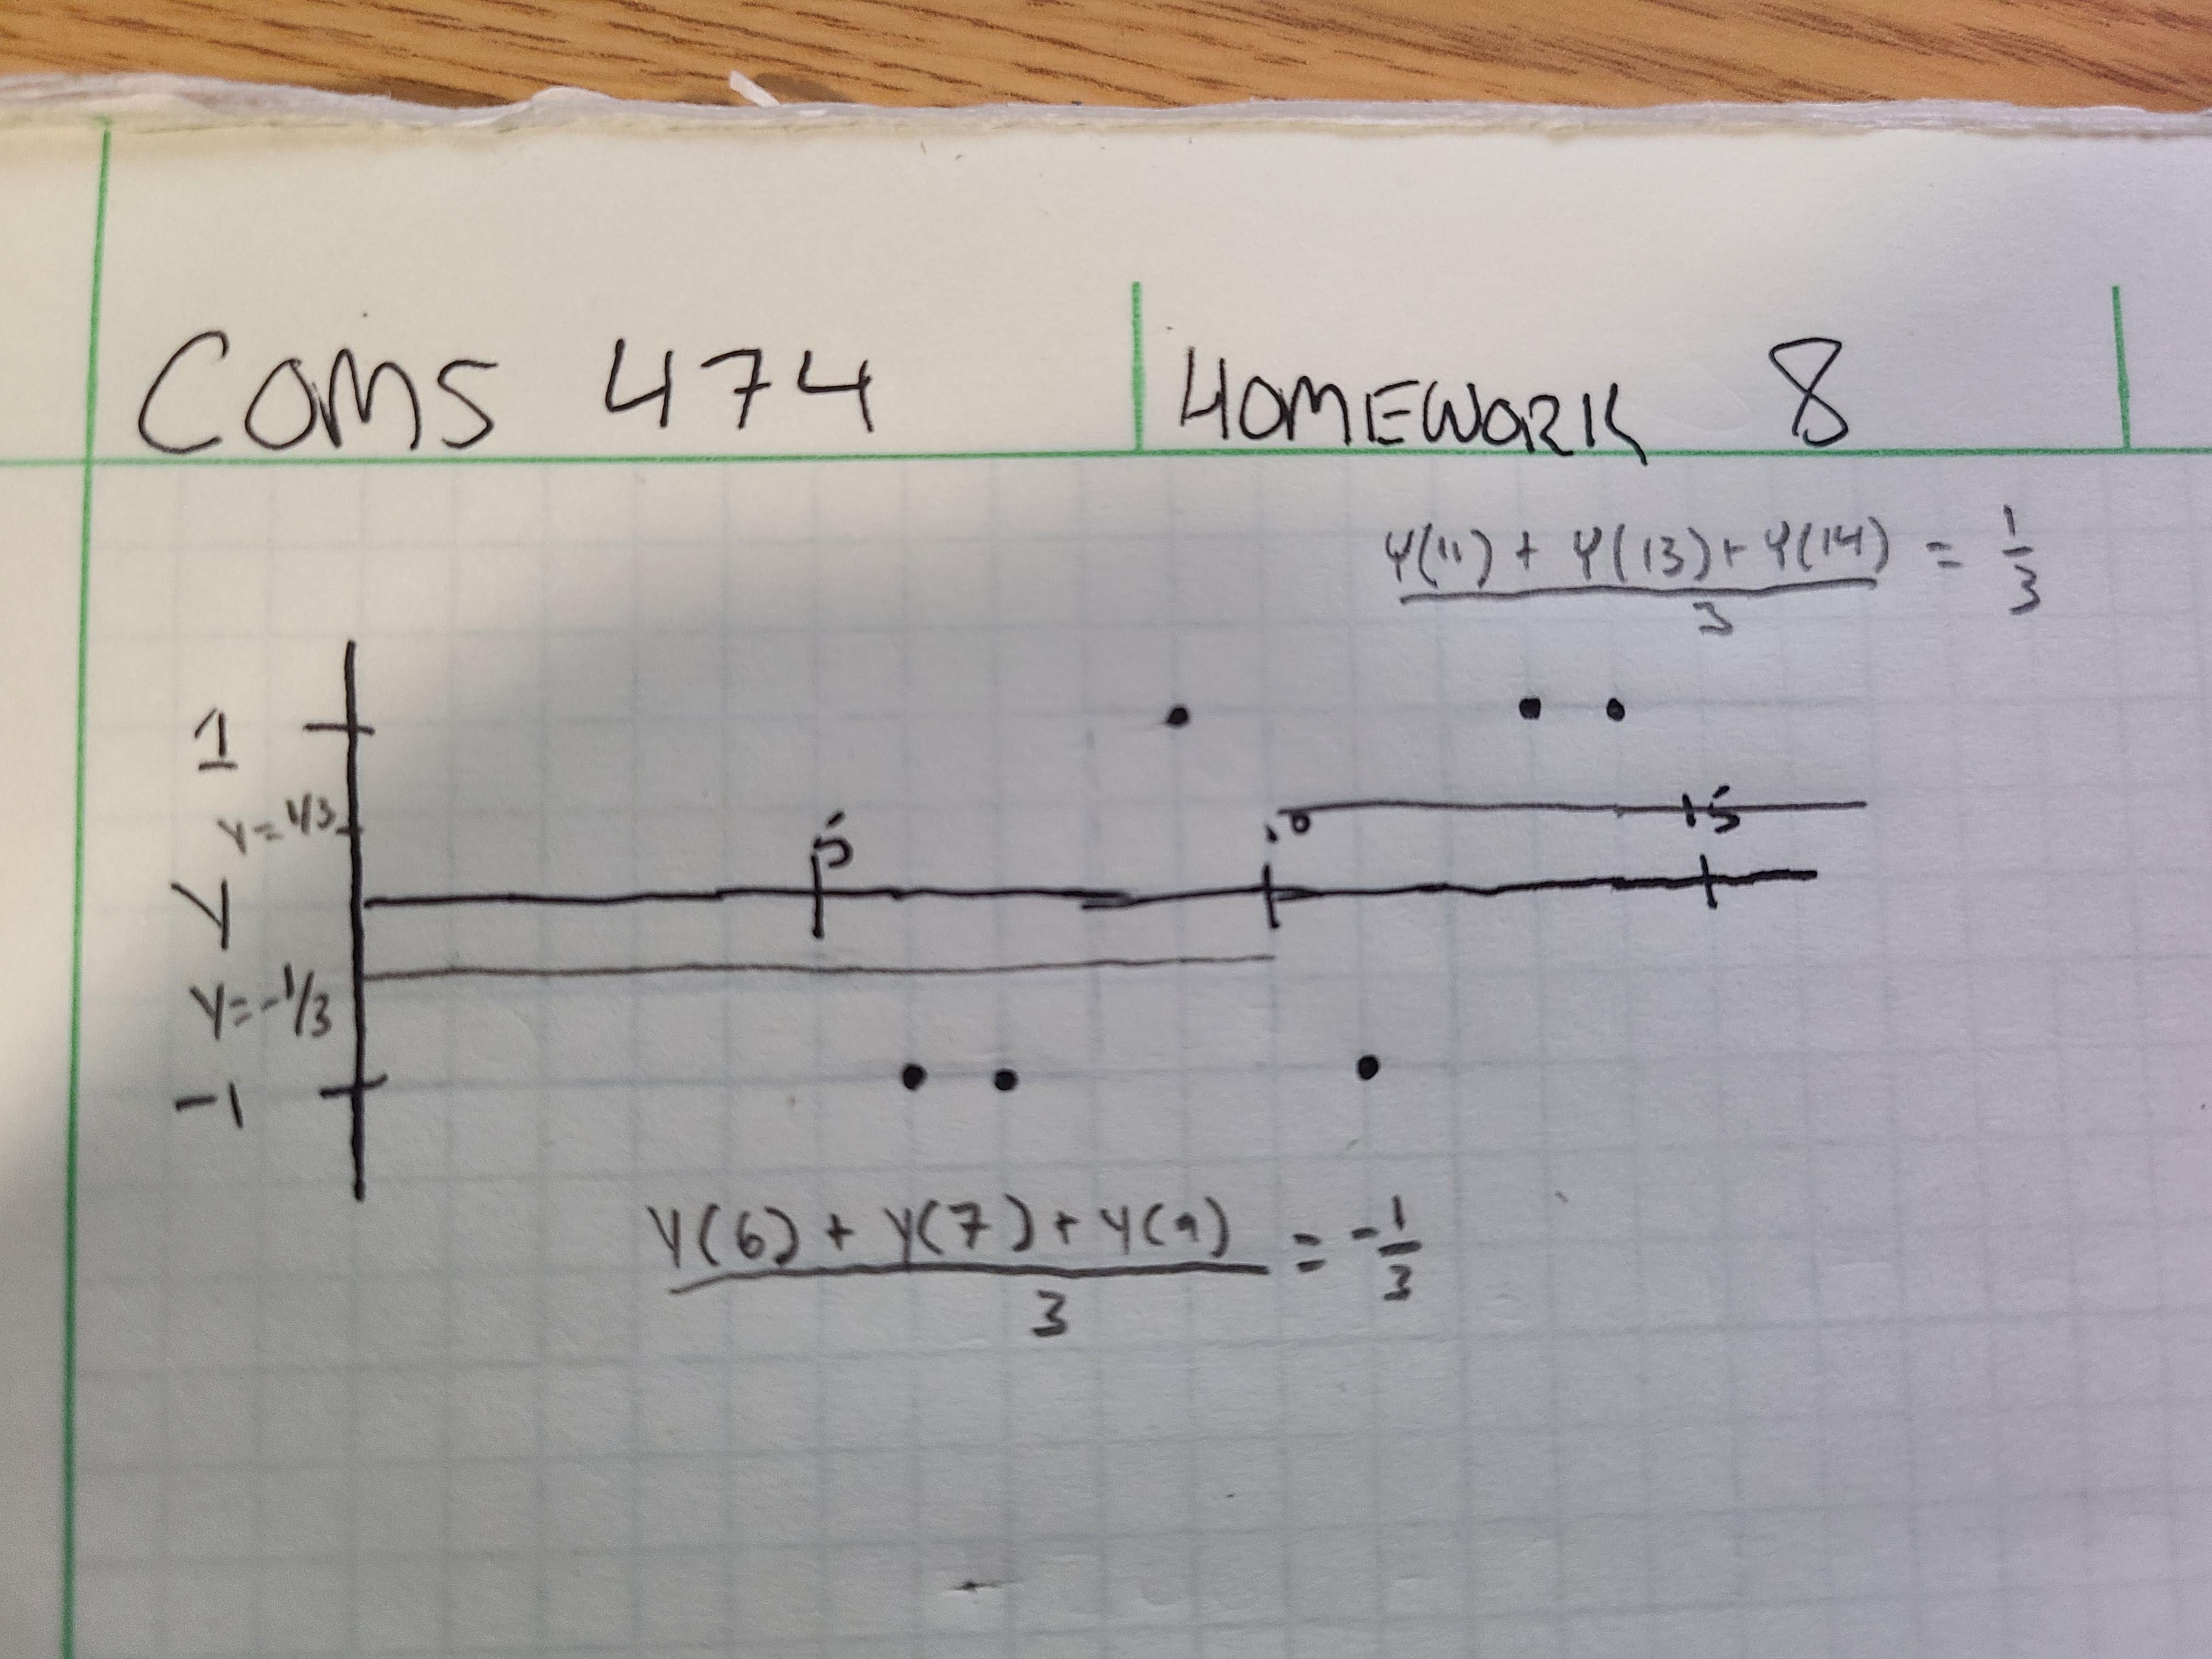
\includegraphics[width=1\textwidth]{p1.c.jpg}

\subsection{D}
Sketch the prediction function $\hat{Y}(x)$ for the $k = 5$ nearest neighbour classifier on the scatter plot. Briefly explain your process.\\
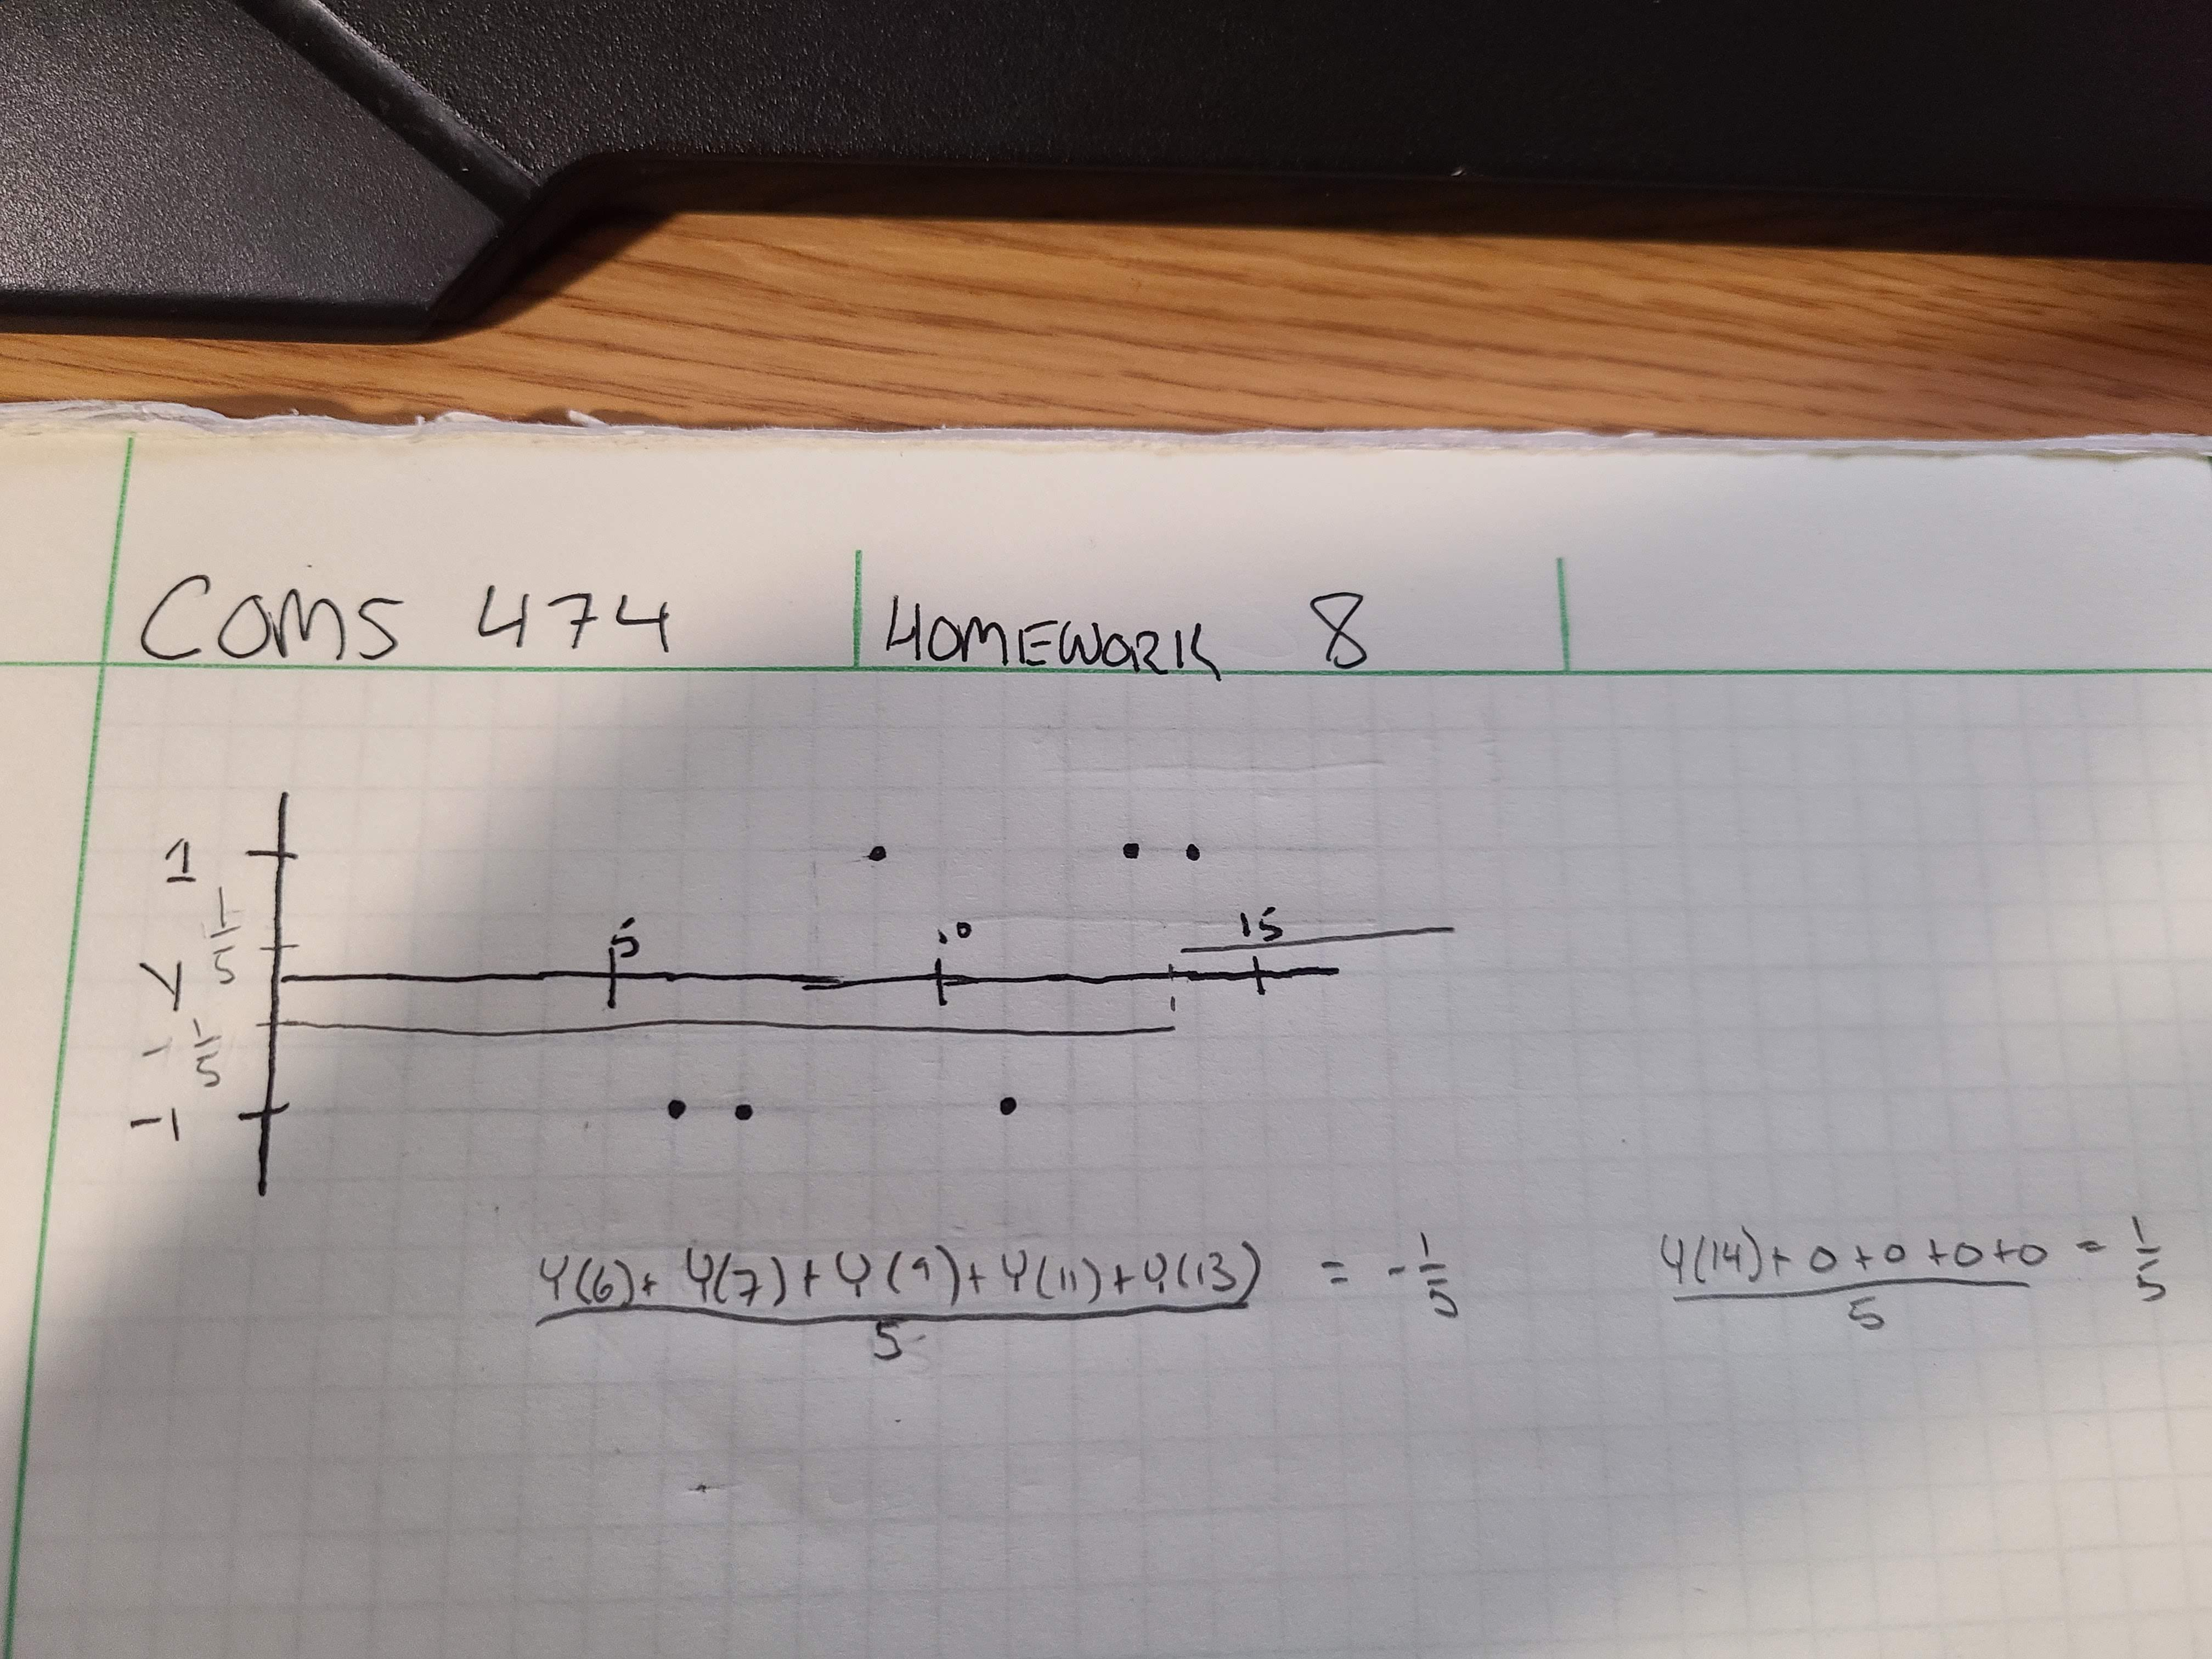
\includegraphics[width=1\textwidth]{p1.d.jpg}

\subsection{E}
Describe what would happen if you tried to use the max margin classifier for this data set.\\
For Max Margin Classifier, if the data is separable, it would result in two parallel lines at $y = +1$ and $y = -1$ that are equally separable.

\pagebreak
\section{Problem 2}
 [20 points; 4 each A-E]\\
For this problem you will fit classifiers to the same data sets you used in the last homework.
\subsection{A}
Copy of Plot:\\
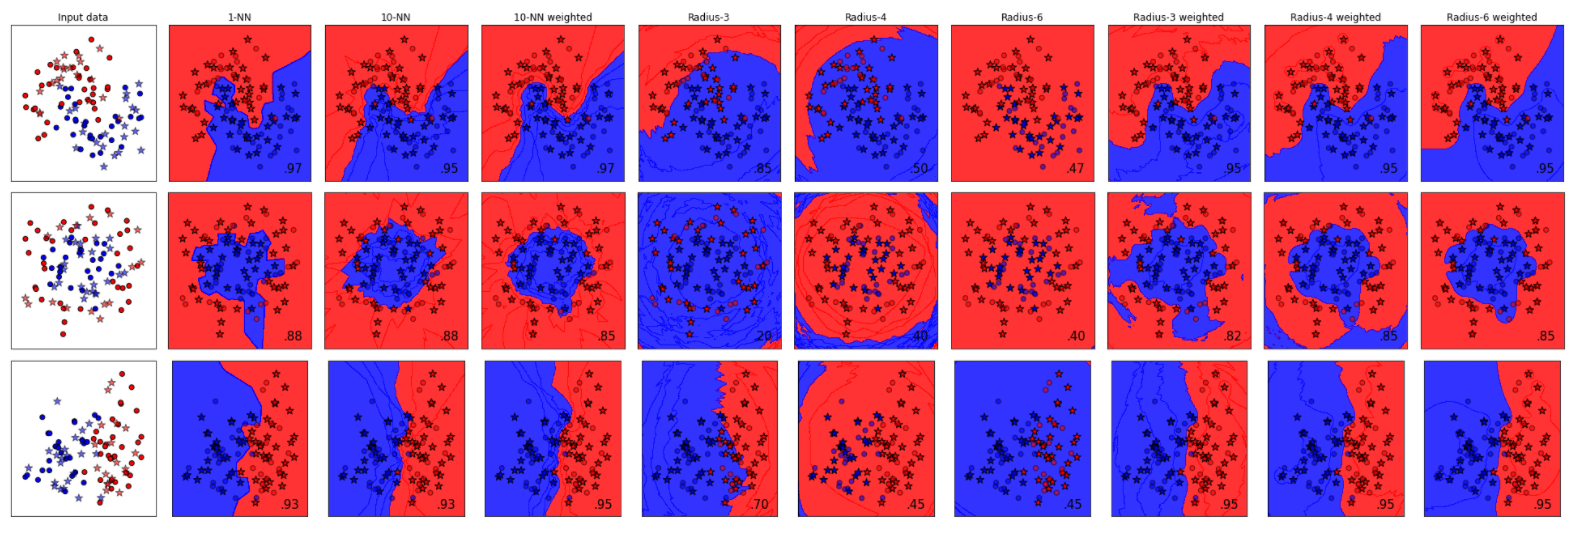
\includegraphics[width=1\textwidth]{p2.a.png}

\subsection{B}
Among the k-nearest neighbour classifiers, do the decision regions seem largely similar or quite different? If quite different, briefly describe the differences.\\\\
The decision regions are largely similar since the radius changes only a little bit for each iteration

\subsection{C}
Among the radius based neighbours classifiers, do the decision regions seem largely similar or quite different? If quite different, briefly describe the differences\\\\
The decision regions that are based of the unweighted radii, they vary significantly when looking at the second and third sets of data, however for all three sets of data for the weighted radii they are very similar bar the outer boarders of the graph on the second set of data.

\subsection{D}
Are the decision regions of the k-nearest neighbour classifiers and the fixed-radius nearest neighbour classifiers largely similar or quite different? If quite different, briefly describe the differences.\\\\
The decision regions are very similar with only signifiant changes on the boundaries of the graph

\subsection{E}
Lastly, briefly discuss which, if any, of the classifiers used in HW7 had similar decision regions to the ones here across all or some of the data sets.\\\\
The support vector that uses a radial basis looks similar, but the most likely reason is because its using a radial basis over a linear one instead. The shape of the models have resemblance, however that is in the nature of classifiers chosen. The others have little to no similarities at all




%--/Paper--
\end{document}